\documentclass[12pt]{article}
\usepackage[brazil]{babel}
\usepackage[T1]{fontenc}
\usepackage[utf8]{inputenc}
\usepackage{amssymb}
\usepackage[pdftex]{graphicx}
\usepackage{listings}
\usepackage{amsmath}
\usepackage{float}
\usepackage{natbib}
\usepackage{amssymb}

\title{Introdução à Física Computacional\\Paradoxo de Parrondo e cadeias de Markov}
\author{Luiz Fernando S. E. Santos\\$N^o$ USP: 10892680 }
\date{Junho de 2019}

\begin{document}
\maketitle
\pagebreak

\section{Cadeias de Markov}

Antes de partirmos para o paradoxo de Parrondo própriamente dito, façamos uma breve análise sobre o principal conceito atuante por trás do inesperado resultado obtido com ele: as \textbf{cadeias de Markov}.\\
\\
Para ilustrar, tomemos o exemplo artificial de um espaço contendo duas marcas de lasanha. Por falta de criatividade e economia de caractéres, vamos chamá-las de marcas \textbf{A} e \textbf{B}.\\
Imagine que uma pesquisa de opinião entre os consumidores assíduos de lasanha revelou que um comprador da marca \textbf{A} tem $80\%$ de chance de, na sua próxima ida ao mercado, comprar novamente a lasanha desta marca (o que, no nosso espaço, implica que há uma chance de $20\%$ dele mudar para a marca \textbf{B}), ao passo que alguém que compra a marca \textbf{B} tem $40\%$ de chance de continuar comprando ela e $60\%$ de chance de mudar para a marca \textbf{A} na próxima. Isso pode ser ilustrado no seguinte esquema:\\

\begin{figure}[H]
\centering
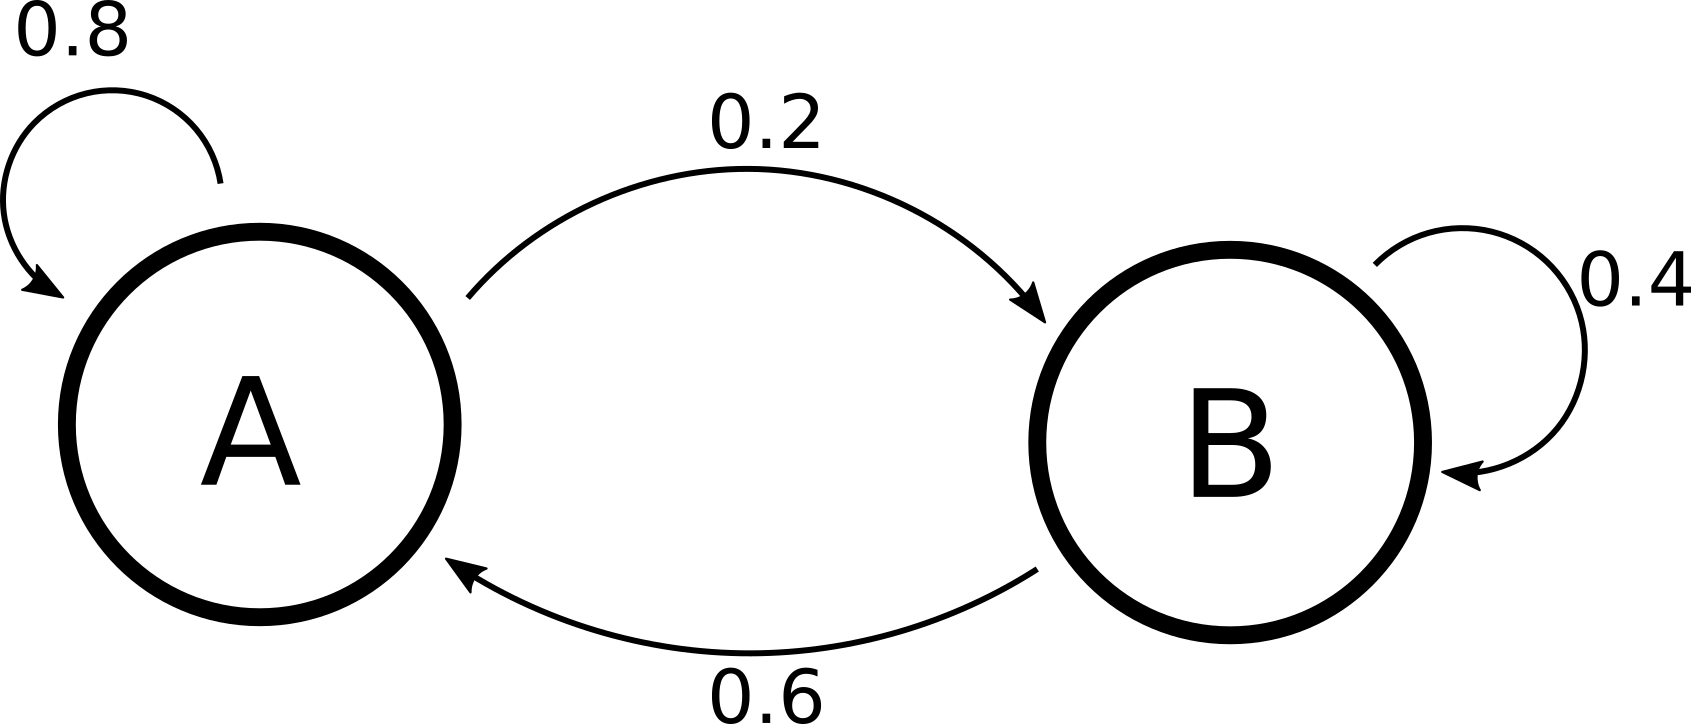
\includegraphics[scale=0.7]{fig1.png}
\end{figure}

Podemos analisar isso da seguinte forma: imagine que todos os compradores de lasanha vão ao mercado uma vez por semana. Se em dado momento $i$ temos um número de consumidores de \textbf{A}, $S_{A, i}$, e de \textbf{B}, $S_{B, i}$, considerando que o número total de consumidores é fixo e normalizado ($S_{A, i} + S_{B, i} = 1$ para todo $i$), na semana seguinte o novo número de compradores de cada marca será igual à soma dos que estão comprando-a novamente com aqueles que acabaram de mudar da outra:

\begin{figure}[H]
\centering
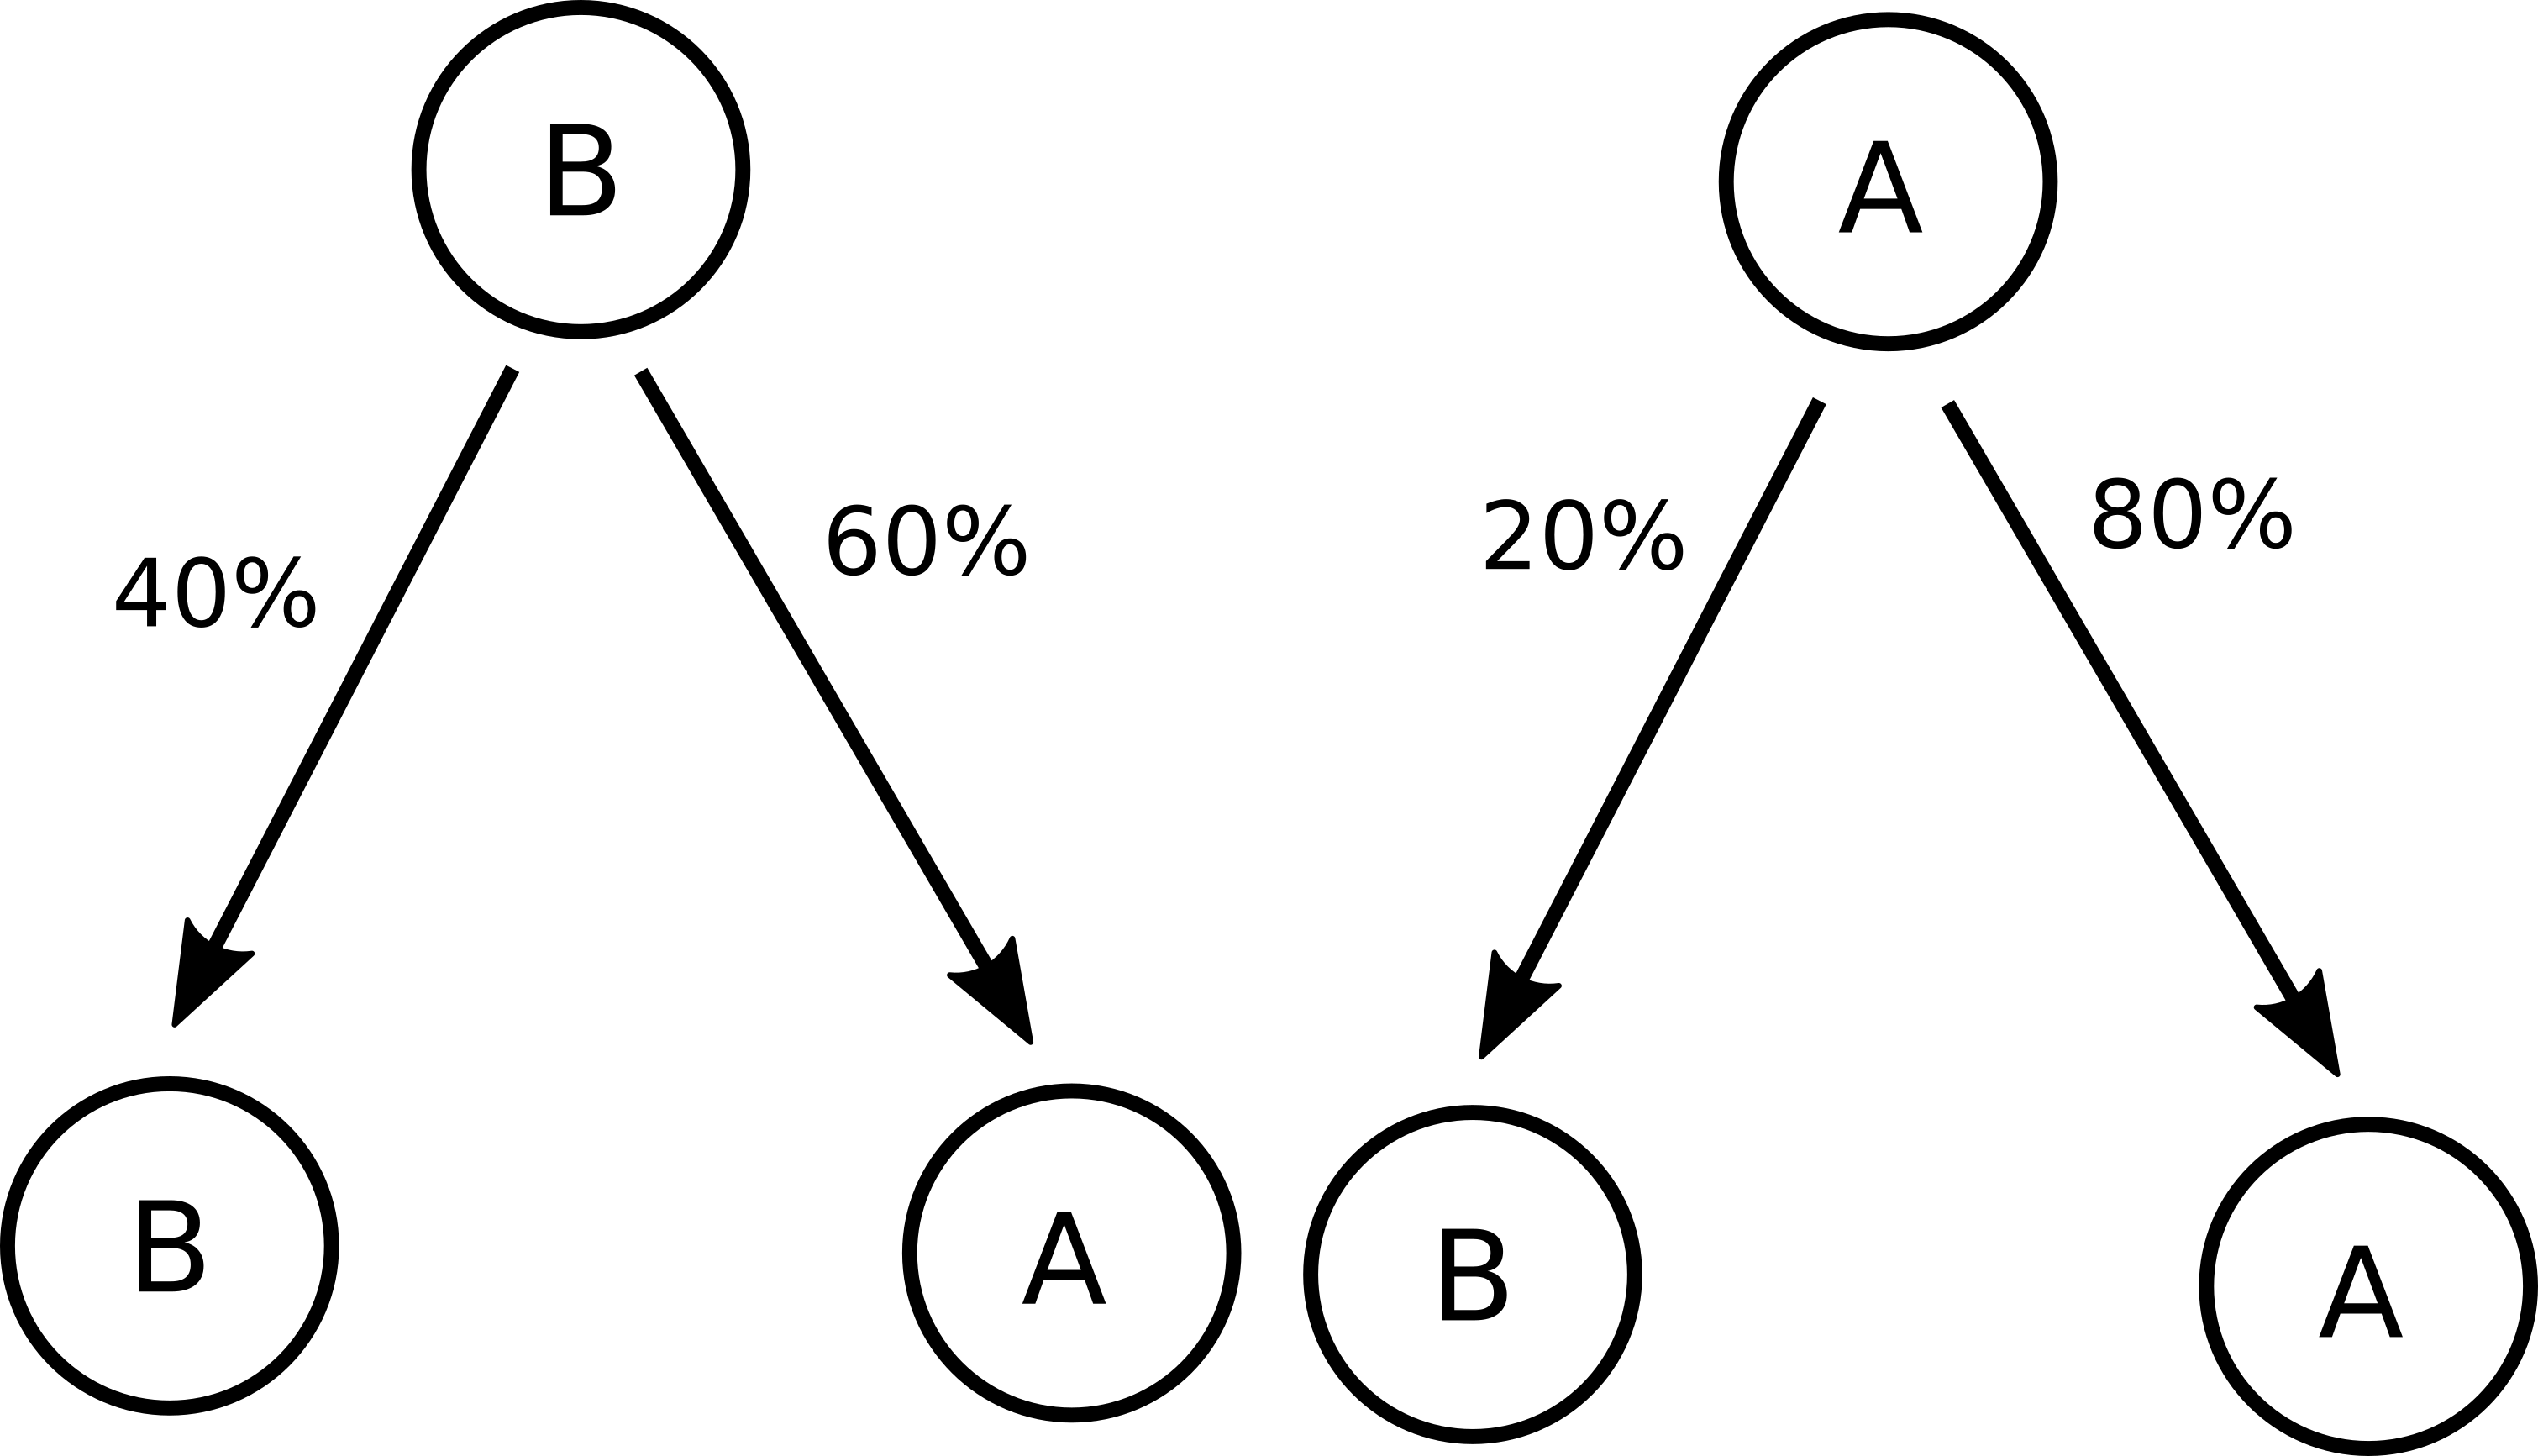
\includegraphics[scale=0.6]{fig2.png}
\end{figure}

Dessa forma, podemos computar uma boa aproximação do novo número de consumidores da seguinte forma:\\
\begin{align*}
	S_{A, i+1} = 0.8S_{A, i} + 0.6S_{B, i}\\
	S_{B, i+1} = 0.2S_{A, i} + 0.4S_{B, i}\\	
\end{align*}

Podemos escrever isso de forma matricial:\\

\begin{equation}
\begin{bmatrix}
S_{A, i} & S_{B, i}
\end{bmatrix}
\begin{bmatrix}
0.8 & 0.2\\
0.6 & 0.4
\end{bmatrix}
=
\begin{bmatrix}
S_{A, i+1} & S_{B, i+1}
\end{bmatrix}
\end{equation}

A matriz quadrada do lado esquerdo da equação é a chamada \textit{matriz de transição} (ou matriz estocástica). Ela possui como linhas o estado atual e nas colunas o próximo estado. No nosso problema, por exempo, o estado atual seria qual marca a pessoa comprou, ao passo que o próximo estado é qual ela vai comprar. Uma pessoa que comprou \textbf{A}, por exemplo, está na primeira linha.\\
Até aqui tratamos $S_A$ e $S_B$ como populações totais. Vamos fazer uma pequena mudança e tratá-los como porcentagens de uma dada população (isso não muda nada nesse problema, mas em casos mais complexos pode ser necessário).\\
Note que se queremos prever qual porcentagem dos consumidores comprou cada marca após duas semanas, simplesmente fazemos:\\

\begin{align*}
\begin{bmatrix}
S_{A, i+2} & S_{B, i+2}
\end{bmatrix} 
=
\begin{bmatrix}
S_{A, i+1} & S_{B, i+1}
\end{bmatrix}
\begin{bmatrix}
0.8 & 0.2\\
0.6 & 0.4
\end{bmatrix}
=
\left(
\begin{bmatrix}
S_{A, i} & S_{B, i}
\end{bmatrix}
\begin{bmatrix}
0.8 & 0.2\\
0.6 & 0.4
\end{bmatrix}
\right)
\begin{bmatrix}
0.8 & 0.2\\
0.6 & 0.4
\end{bmatrix}
\end{align*}
E por comutatividade:

$$
\begin{bmatrix}
S_{A, i} & S_{B, i}
\end{bmatrix}
\left(
\begin{bmatrix}
0.8 & 0.2\\
0.6 & 0.4
\end{bmatrix}
\begin{bmatrix}
0.8 & 0.2\\
0.6 & 0.4
\end{bmatrix}
\right)
=
\begin{bmatrix}
S_{A, i+2} & S_{B, i+2}
\end{bmatrix}
$$

Generalizando, se queremos saber saber as populações em um instante $i + n$, simplesmente fazemos:

\begin{equation}
\begin{bmatrix}
S_{A, i} & S_{B, i}
\end{bmatrix}
\begin{bmatrix}
0.8 & 0.2\\
0.6 & 0.4
\end{bmatrix}^n
=
\begin{bmatrix}
S_{A, i+n} & S_{B, i+n}
\end{bmatrix}
\end{equation}

Vamos sair um pouco do nosso problema original e fazer uma generalização dos conceitos que temos até agora: definimos a matriz estocástica como aquela que representa as transições de estado em uma cadeia de Markov. Seus elementos são numeros reais não negativos, que representam as probabilidades. Dependendo da representação escolhida, ela pode ter a soma de cada linha ou coluna (em algus casos, ambos) iguais à 1. Isso vai depender se ela é \textit{direita} ou \textit{esquerda}, o que básicamente indica "por qual lado" ela está multiplicando o \textbf{vetor estocástico}. No nosso caso, estamos e vamos continuar usando a representação direita da matriz estocástica, mas podemos transicionar fácilmente entre as representações através da identidade:
\begin{equation}
(vM)^{\dagger} = M^{\dagger} v^{\dagger}
\end{equation}
Onde $M$ é uma matriz e $v$ um vetor. Como seus elementos são reais, o operador adjunto simplesmente indica a transposição.\\
\\
Algo muito interessante vem dessa representação. Voltando à visualização das lasanhas, imagine que queremos saber se, em algum momento, a porcentagem de clientes de cada marca irá convergir para algum valor. Isso seria o equivalente à dizer que o próximo estado será igual ao atual:

$$
\begin{bmatrix}
S_{A, i} & S_{B, i}
\end{bmatrix}
\begin{bmatrix}
0.8 & 0.2\\
0.6 & 0.4
\end{bmatrix}
=
\begin{bmatrix}
S_{A, i} & S_{B, i}
\end{bmatrix}
$$

Note que isso é o equivalente à dizer que o vetor estocástico em questão é um autovetor da matriz estocástica, com autovalor 1. Ficamos com o sistema:

$$
\left\{
\begin{array}{ll}
-0.2 S_{A, i} + 0.6 S_{B, i} = 0\\
0.2 S_{A, i}  - 0.6 S_{B, i} = 0\\
S_{A, i} + S_{B, i} = 1
\end{array}\right.
$$

Temos aqui que a solução para esse sistema linear é $S_{A, i} = 0.75$, $S_{B, i} = 0.25$. Ou seja, $\begin{bmatrix} 0.75 & 0.25 \end{bmatrix}$ é o \textit{estado estável} dessa matriz de Markov.\\ 
Podemos ilustrar isso iterando e equação [1] para um certo valor de $i$ e ver o comportamento de $S_{A, i}$ e $S_{B, i}$:

\begin{figure}[H]
\centering
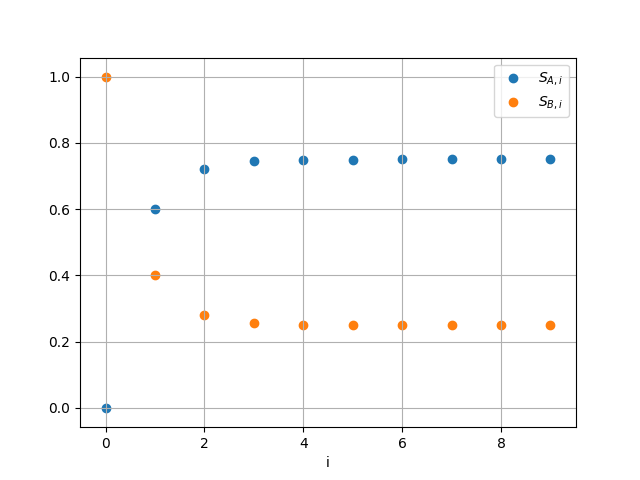
\includegraphics[scale=0.55]{graph1.png}
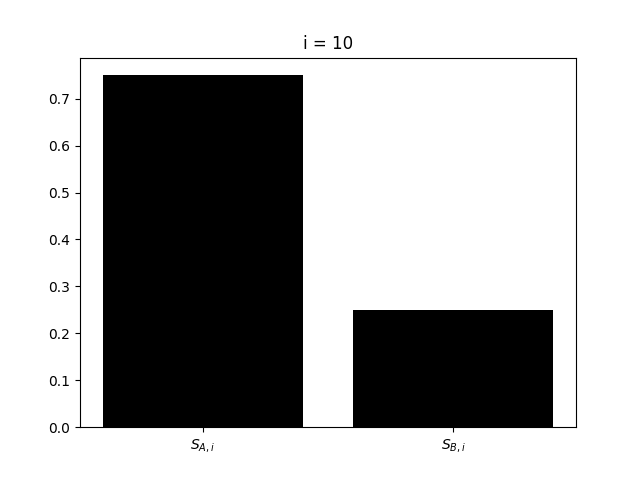
\includegraphics[scale=0.55]{graph2.png}
\caption{Gráficos da convergência do vetor de probabilidades.}
\end{figure}

No caso ilustrado acima tomamos um vetor de probabilidade inicial qualquer $\begin{bmatrix} 0.0 & 1.0 \end{bmatrix}$. Pode haver dúvida quanto à se essa convergência seria diferente se o vetor inicial fosse outro. Acontece que haver \textit{outro} estado estável implicaria que o autovalor $1$ referente á matriz estocástica é degenerado (isto é, admite dois ou mais autovetores não paralelos). Isso pode ser mostrado facilmente que não é possível para o caso de uma matriz de ordem 2:
\begin{equation}
\begin{bmatrix} v_1 & v_2 \end{bmatrix}
\begin{bmatrix}
x & y\\
z & k
\end{bmatrix}
=
\begin{bmatrix} v_1 & v_2 \end{bmatrix}\\
\Rightarrow 
\left\{
\begin{array}{ll}
xv_1 + zv_2 - v_1 = 0\\
yv_1 + kv_2 - v_2 = 0\\
\end{array}\right.
\end{equation}
Mas pela definição:
\begin{equation}
\left\{
\begin{array}{ll}
x + y = 1\\
z + k = 1\\
v_1 + v_2 = 1
\end{array}\right.
\end{equation}
Substituindo [5] em [4], ficamos com:
\begin{equation}
\left\{
\begin{array}{ll}
xv_1 + zv_2 - v_1 = 0\\
v_1 + v_2 = 1
\end{array}\right.
\end{equation}
Temos duas variáveis e duas equações lineares. Com exceção de um caso especial, o autovalor 1 admite um e \textbf{apenas} um autovetor. Vale comentar que, se $x = 0$ e $z = 1$ ou vice-versa, algo interessante acontece:

\begin{figure}[H]
\centering
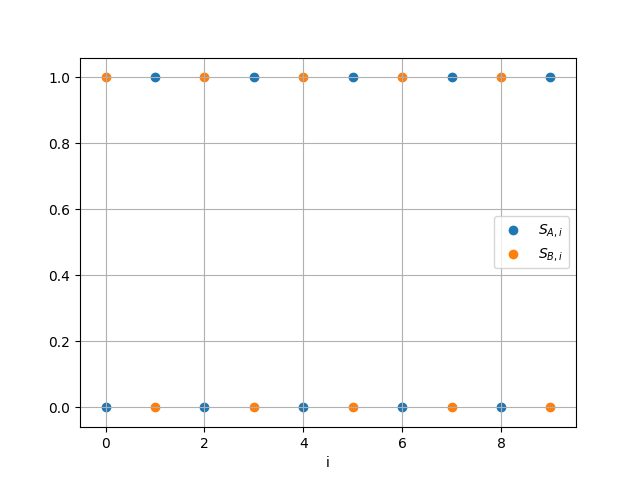
\includegraphics[scale=0.6]{graph3.png}
\caption{Caso $x = 0$ e $z = 1$.}
\end{figure}

Nesse caso da imagem, embora haja apenas um autovetor ($\begin{bmatrix} 0.5 & 0.5 \end{bmatrix}$), a iteração não alcança um estado estático se o vetor inicial não é o próprio autovetor. No outro caso citado, ficamos com a matriz identidade e dizemos que 1 é um autovalor degenerado, e seu \textit{autoespaço associado} é a circunferência de raio 1 na origem. Para maiores dimensões há outras complicações.\\
\\
O motivo pelo qual perdemos todo esse tempo para desenvolver estes conceitos ficará mais claro a seguir.

\section{O paradoxo de Parrondo}

O paradoxo proposto por Juan Parrondo afirma que, havendo dois jogos (ou quaisquer outros sistemas probabilísticos) \textbf{não relacionados}, os quais jogados separadamente as chances estão sempre contra o jogador, é possível que, jogados em conjunto, resultem em um resultado favorável à vitória.\\
\\
Para visualizarmos essa ideia, vamos tomar dois jogos simples: o primeiro é a clássica roleta.

\begin{figure}[H]
\centering
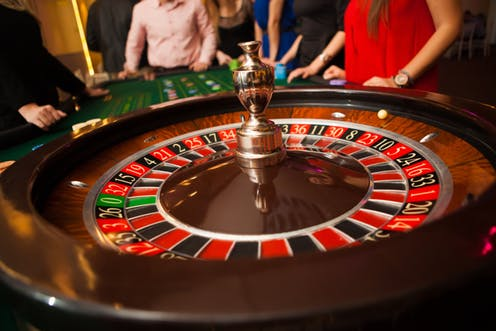
\includegraphics[scale=0.55]{roleta.jpg}
\caption{Roleta de cassino.}
\end{figure}

Ela é jogada escolhendo uma entre as duas cores (vermelho ou preto). Imagine que nossa roleta possui $67$ casas no total: $33$ vermelhas, $33$ pretas e uma verde (a neutra). A chance de vitória é de $33$ entre as $67$ casas, aproximadamente  $49.5\%$. Isso implica que há uma chance de derrota $1\%$ maior que a de vencer. Imagine que um jogador desavisado decide jogar algumas vezes a roleta. Em um tempo discreto, tomando que ele ganhe R$\$1,00$ se vencer e perca a mesma quantia se perder, seu dinheiro total em relação ao tempo será algo como:

\begin{figure}[H]
\centering
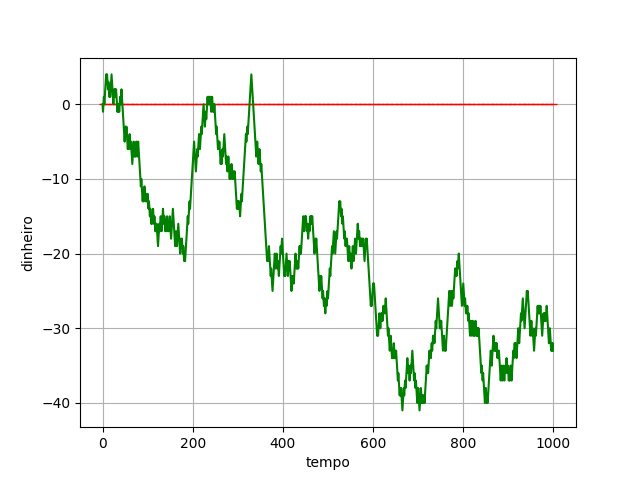
\includegraphics[scale=0.7]{graph4.png}
\caption{Gráfico de dinheiro em relação ao tempo para certo jogo.}
\end{figure}

Podemos ver o histograma do dinheiro ao final do jogo:

\begin{figure}[H]
\centering
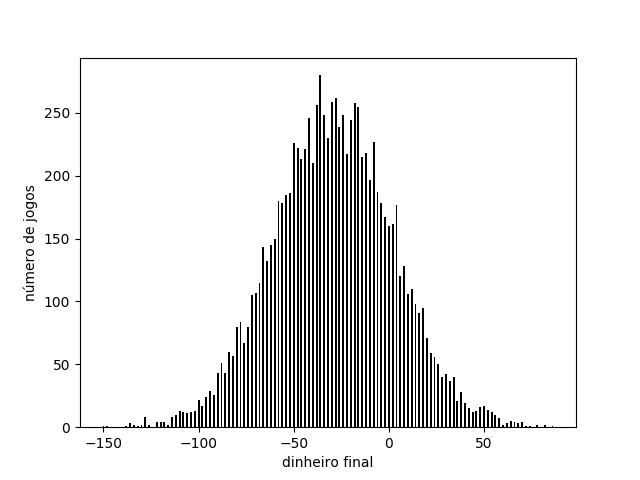
\includegraphics[scale=0.8]{graph5.png}
\caption{Histograma para dez mil jogos, com mil jogadas cada.}
\end{figure}

O gráfico é bonito, mas as chances para o jogador não. É visível que as chances de se ganhar alguma coisa com esse jogo não são favoráveis.\\
\\
O segundo jogo é um pouco mais complicado. Tomemos o seguinte cenário: se o dinheiro que o jogador possue é um mútiplo de três, ele puxa uma carta em um deck de $200$. Caso essa carta seja uma das $19$ especiais, ele ganha 1 (um) real. Caso contrário, ele perde esse valor.\\
Não é difícil perceber que esse é um jogo em que se perde! $19$ cartas entre $200$ resulta em uma chance de vitória de apenas $9.5\%$. Mas tem um detalhe: se o dinheiro do jogador \textbf{não} for um múltiplo de três, ele tem uma boa vantagem: uma moeda enviesada é jogada e suas chances se tornam de $74.5\%$ de uma vitória.\\
Pode-se até pensar que isso seja vantajoso para o jogador, uma vez que alguém pode, equivocadamente, deduzir que ele tem só $\frac{1}{3}$ de chance de jogar o jogo ruim.
\\
Porém vamos parar e analisar um pouco mais friamente o que está acontecendo:\\
Tomemos o dinheiro total $n \in \mathbb{Z}$, a condição para jogar o jogo ruim é $n \in \{..., -6, -3, 0, 3, 6, ...\}$, o conjunto dos números múltiplos de 3.\\
Vamos dividir os valores possíveis de $n$ em três grupos diferentes: 
\begin{align*}
P_{1} = \{..., -5, -2, 1, 4, ...\}\\
P_{2} =  \{..., -4, -1, 2, 5, ...\}\\
P_{3} = \{..., -3, 0, 3, 6, ...\}
\end{align*}

Bom, se $n \in P_1$ ou $n \in P_2$, fazemos o jogo bom e, caso contrário, o ruim.\\
Agora vamos aplicar o que vimos a respeito das cadeias de Markov. Podemos dizer que $n$ está em um dos três diferentes estados (representados aqui pelos conjuntos), e sua chance de passar de um para o outro pode ser representada assim, dependendo das chances de ganhar ou perder:

\begin{figure}[H]
\centering
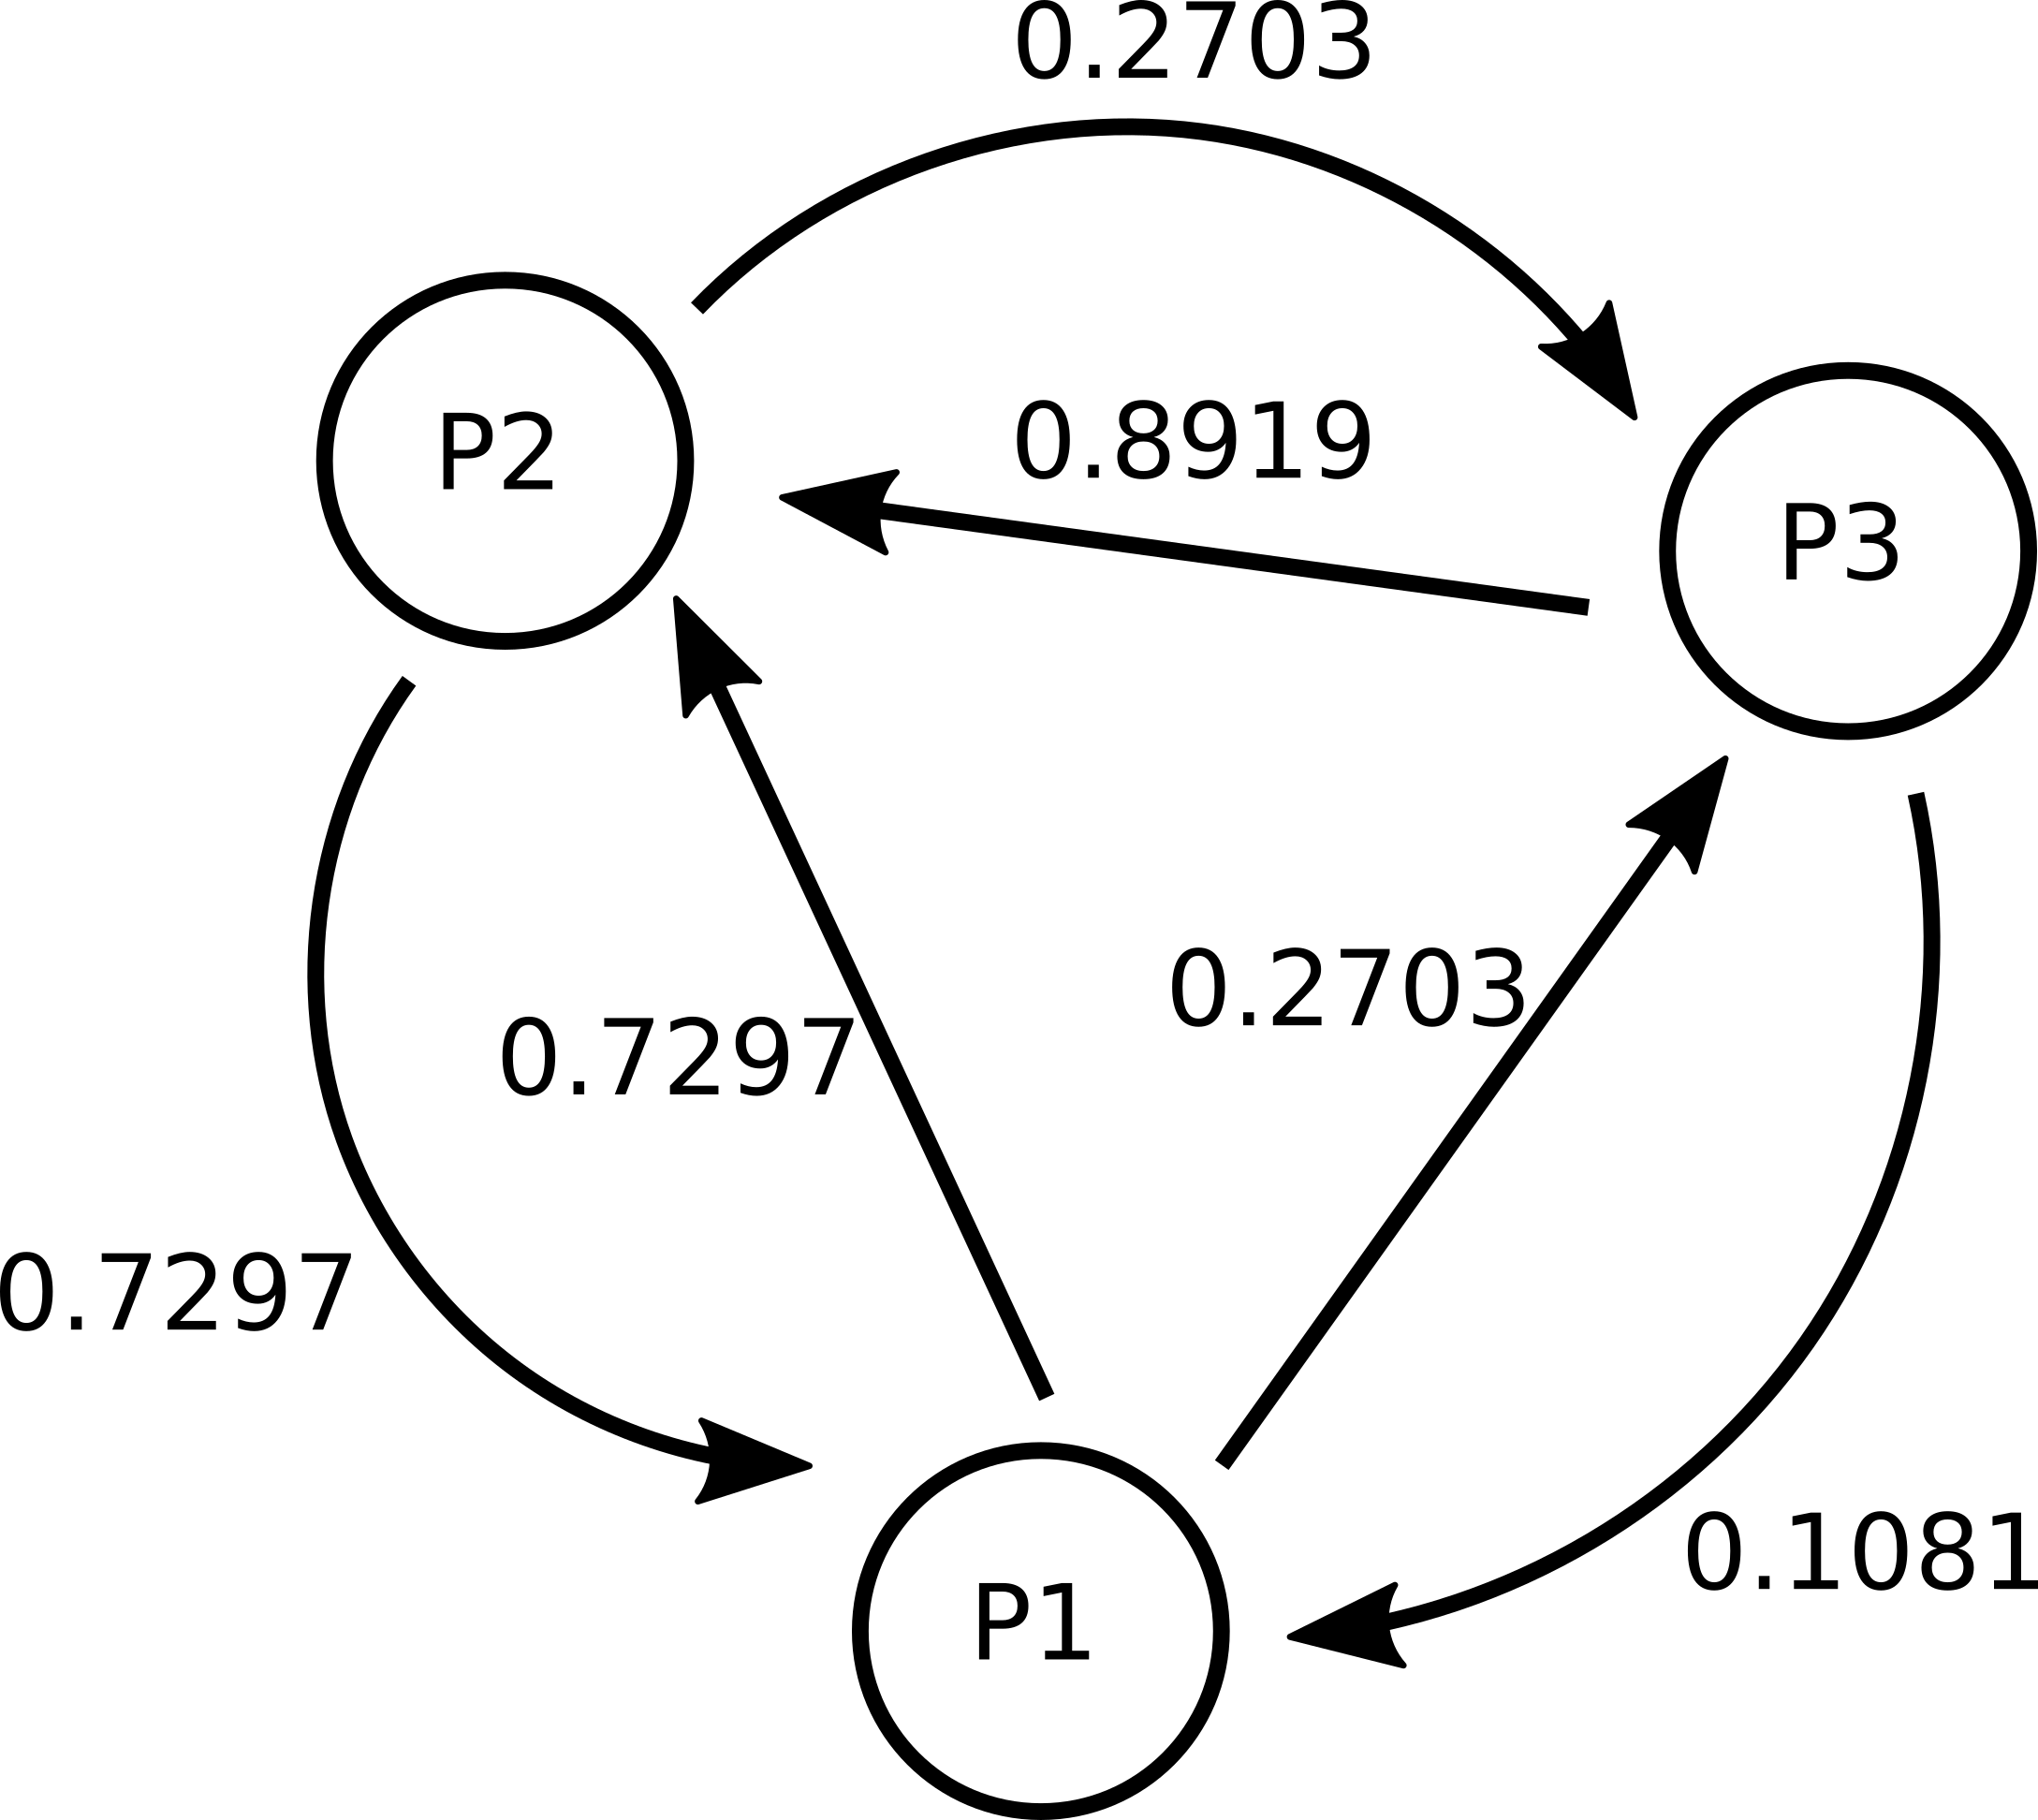
\includegraphics[scale=0.7]{fig3.png}
\end{figure}

Montando a matriz estocástica desse sistema, obtemos:

$$
M = 
\begin{bmatrix}
0 & 0.745 & 0.255\\
0.255 & 0 & 0.745\\
0.095 & 0.905 & 0
\end{bmatrix}
$$
Podemos visualizar a convergência para o estado estável $v = \begin{bmatrix} \pi_1 & \pi_2 & \pi_3 \end{bmatrix} $ iterando:

\begin{figure}[H]
\centering
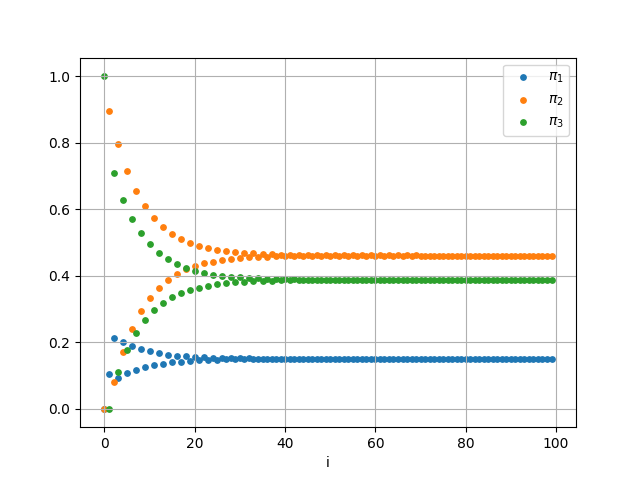
\includegraphics[scale=0.55]{graph6.png}
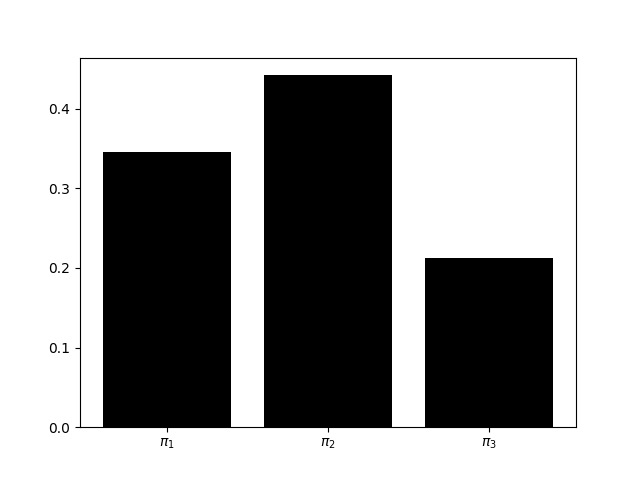
\includegraphics[scale=0.55]{graph7.png}
\caption{Convergência do vetor de probabilidades para o estado estável.}
\end{figure}

Assim obtemos que $v = \begin{bmatrix} 0.1543 & 0.4621 & 0.3836 \end{bmatrix}$ é o estado estável dessa matriz estocástica. Para acharmos a chance média de vitória nesse jogo, fazemos:\\

$$
\rho = 0.745\pi_1 + 0.745\pi_2 + 0.095\pi_3 
$$

Note que os $\pi_i$ representam com qual frequência estamos em cada estado, e o número multiplicando é a chance de ganhar nesse estado. Diferente do que se pode imaginar, é bem diferente de $\frac{1}{3}$ para cada.
Substituindo os valores encontrados de $v$, temos $\rho = 0.4956$, a chance de ganharmos nesse jogo. Isso quer dizer que a chance de vitória ao longo prazo ainda está contra o jogador.\\
Podemos confirmar isso pelo histograma:

\begin{figure}[H]
\centering
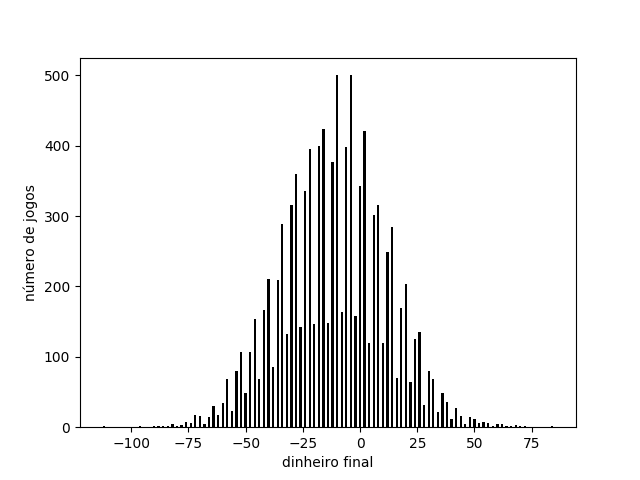
\includegraphics[scale=0.8]{graph8.png}
\caption{Histograma do segundo jogo, para dez mil jogos, com mil jogadas cada.}
\end{figure}

Então continuamos na desvantagem. Dois jogos de azar independentes, nos quais ambos as chances estão contra o jogador.\\
A parte interessante, porém, começa agora:\\
\\
Imagine que, antes decidir qual dos dois jogar, o jogador joga uma moeda justa. Se cair coroa, ele vai para o primeiro jogo. Caso contrário ele vai para o segundo.\\
Não parece nada demais, mas essa pequena mudança tem reflexos surpreendentes no resultados. Vamos análisar visualmente o que acontece:

\begin{figure}[H]
\centering
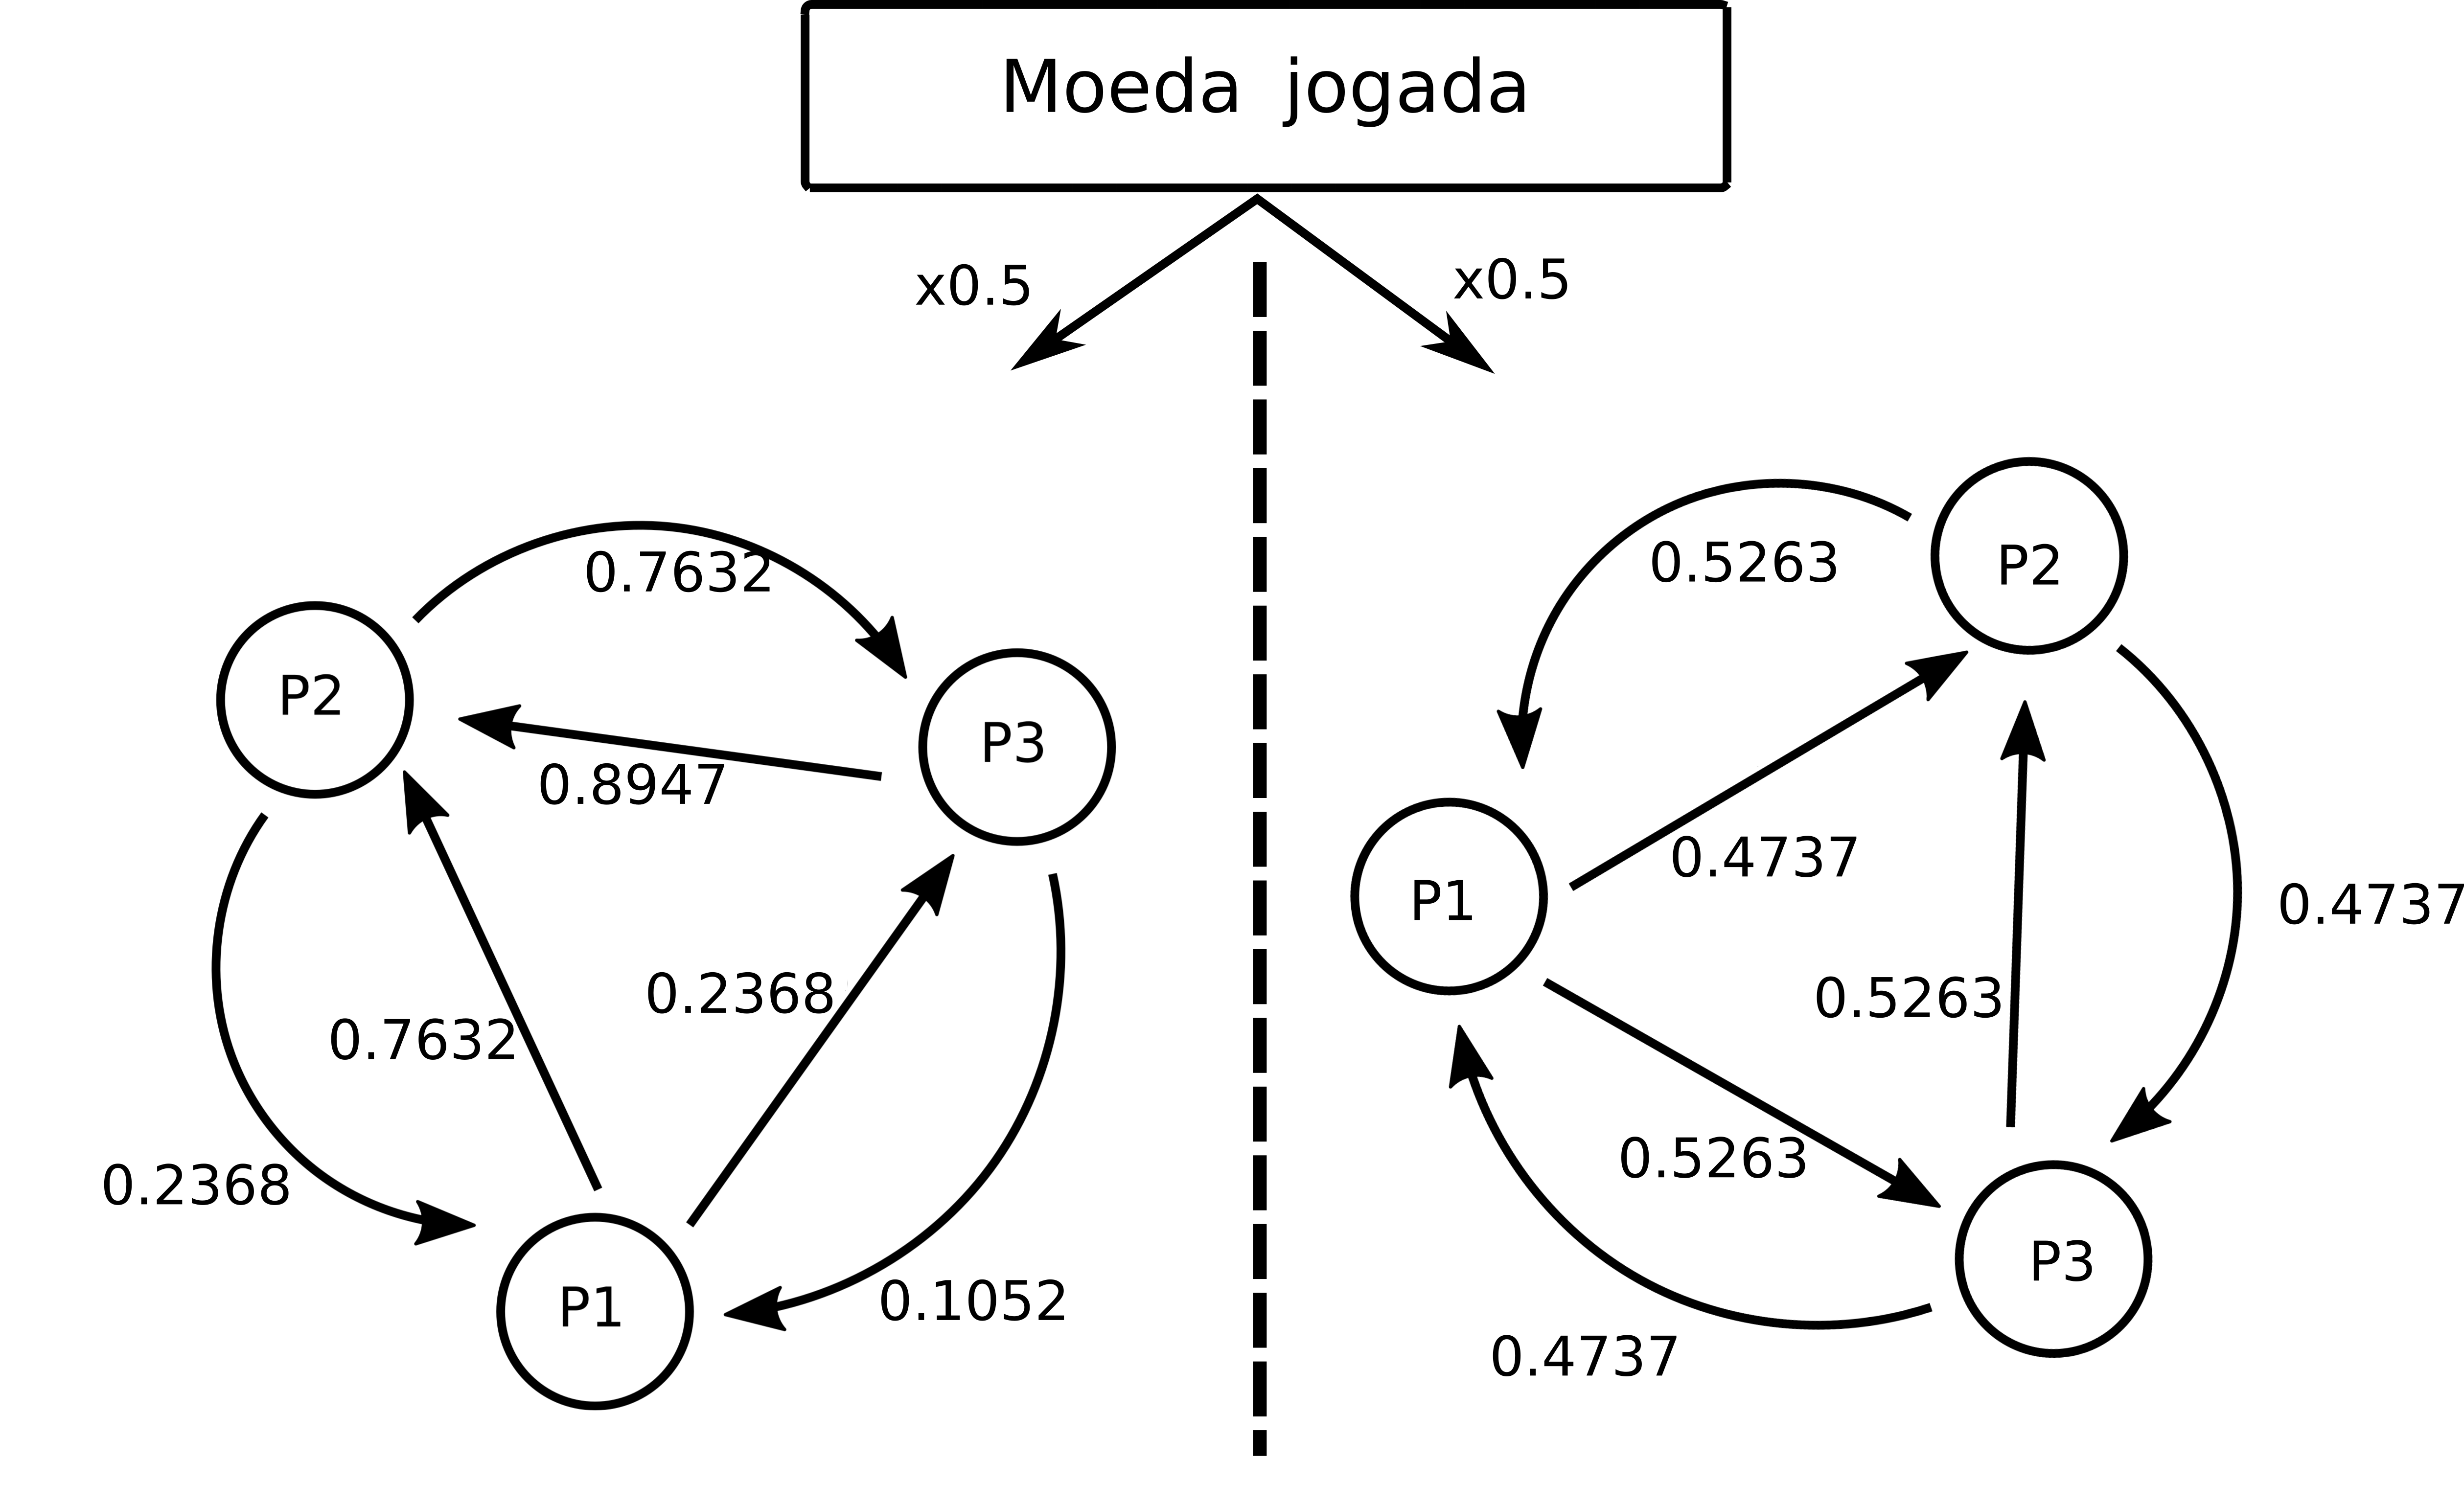
\includegraphics[scale=0.5]{fig4.png}
\end{figure}

Para montarmos a matriz estocástica desse sistema, simplesmente consideramos \textit{metade} da probabilidade de que cada transição de estado ocorra. Dessa forma, temos:\\

$$
M = 
\begin{bmatrix}
0 & \frac{1}{2}(0.745 + 0.495)  & \frac{1}{2}(0.255 + 0.505)\\
\frac{1}{2}(0.255 + 0.505) & 0 & \frac{1}{2}(0.745 + 0.495)\\
\frac{1}{2}(0.095 + 0.495) & \frac{1}{2}(0.909 + 0.505) & 0
\end{bmatrix}
$$

Vamos ver a convergência dela:

\begin{figure}[H]
\centering
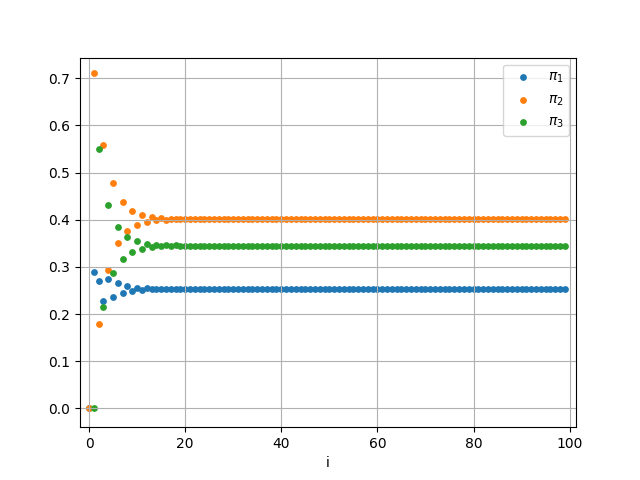
\includegraphics[scale=0.55]{graph9.png}
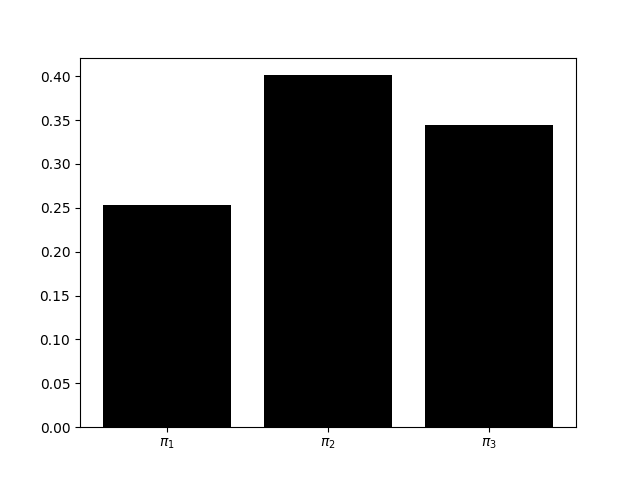
\includegraphics[scale=0.55]{graph10.png}
\caption{Convergência do vetor de probabilidades para o estado estável da nova matriz estocástica.}
\end{figure}

Nosso novo vetor do estado estático é: $v = \begin{bmatrix} 0.2541 & 0.4008 & 0.3451 \end{bmatrix}$. Dessa forma, a probabilidade de vitória é\\
$$
\rho = \frac{1}{2}[(0.745 + 0.495)\pi_1 + (0.745 + 0.495)\pi_2 + (0.095 + 0.495)\pi_3]
$$\\
Isso nos dá $\rho = 0.5078$, ou $50,78\%$ de chance de vitória! Analisando o histograma desse caso:


\begin{figure}[H]
\centering
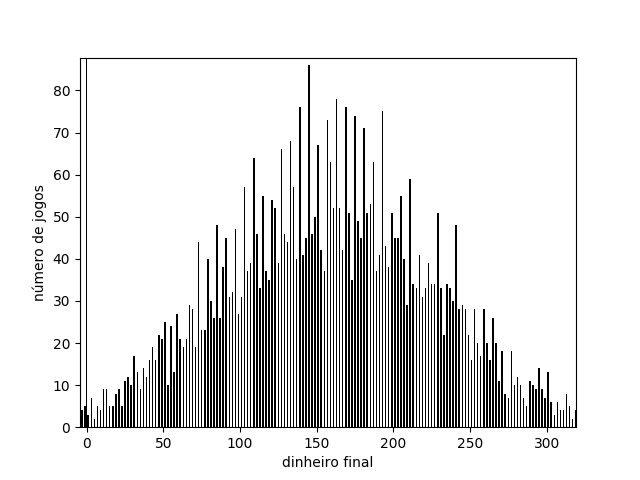
\includegraphics[scale=0.65]{graph11.png}
\caption{Histograma o dinheiro ao final do jogo para o caso dos jogos em conjunto.}
\end{figure}

Vamos ver o que está acontecendo em cada jogo com um pouco mais de precisão:


\begin{figure}[H]
\centering
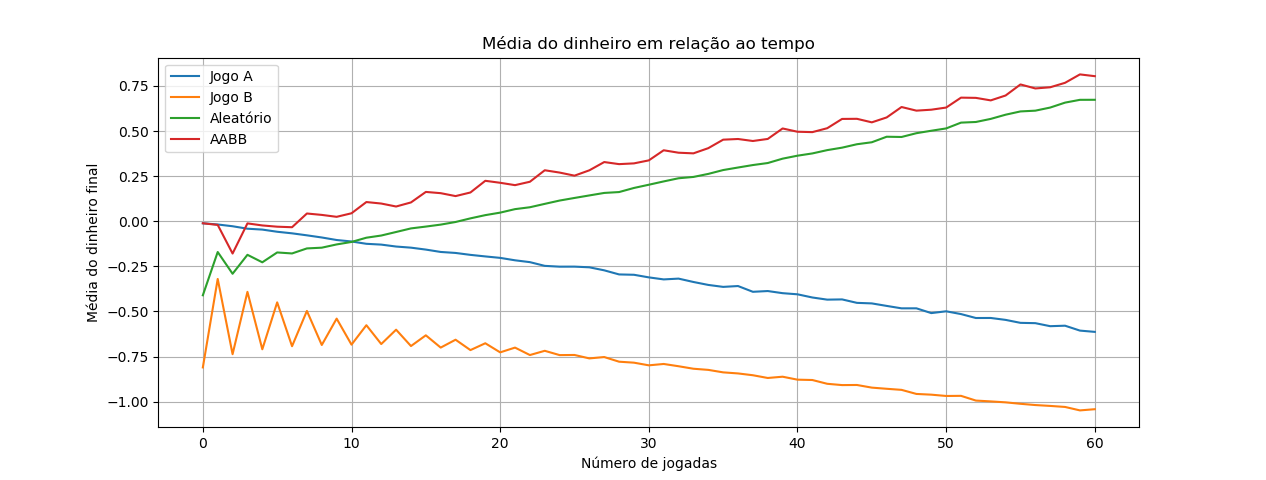
\includegraphics[scale=0.5]{graph12.png}
\caption{Gráfico da média do dinheiro ao final do jogo em função do número de jogadas.}
\end{figure}

De maneira mais geral, pode-se verificar a ocorrência desse paradoxo para dois jogos cujo viés é igual à um certo $\epsilon$ (razoávelmente pequeno) contra o jogador, o segundo jogo contando com a existência de um loop de ordem $m > 2$, $m \in \mathbb{Z}$ e positivo. No nosso caso, usamos $m = 3$, isto é, os jogos se repetem após $m$ vitórias ou derrotas seguidas. Vale ressaltar que não necessáriamente o número de estados é igual à ordem do loop! Eles podem ser definidos como se achar melhor para trabalhar.

\section*{Bibliografia}
\begin{enumerate}
	\item G. P. Hammer, D. Abbot, Losing strategies can win
by Parrondo’s paradox, Nature, volume 402, página 864 (1999)

	\item G. P. Hammer, D. Abbot, Parrondo’s Paradox, Statistical Science, Vol. 14, No. 2, 206 - 203, (1999)

	\item L. Saloff-Coste, Lectures on Finite Markov Chains, Instituto de Matemática e Estatísca, Universidade de São Paulo
	
	\item A. Tolver, An Introduction to Markov Chains, Department of Mathematical Sciences, University of Copenhagen
\end{enumerate}

\end{document}
